\documentclass[aspectratio=169]{beamer}

\makeatletter
\def\input@path{{theme/moloch/}{theme/}}
\makeatother
\usetheme[
  sectionpage=none,
  subsectionpage=none,
  block=fill,
  progressbar=frametitle,
  titleformat=regular
]{moloch}

\usepackage{amsmath}
\usepackage{amssymb}
\usepackage{booktabs}
\usepackage{graphicx}
\usepackage[version=4]{mhchem}
\usepackage{siunitx}
\usepackage{tikz}
\usetikzlibrary{arrows.meta,positioning,calc,shapes.geometric}
\usepackage{pgfplots}
\usepackage{pgfpages}
\pgfplotsset{compat=1.18}

\definecolor{netlgreen}{RGB}{137,190,49}
\definecolor{netlnavy}{RGB}{20,31,46}
\definecolor{netlteal}{RGB}{20,101,116}
\definecolor{netlgray}{RGB}{92,103,112}
\definecolor{netlmist}{RGB}{238,246,242}
\definecolor{netlwarning}{RGB}{175,88,28}

\molochset{
  colors/theme=highcontrast,
  colors/variant=light,
  titleformat section=allcaps,
  progressbar linewidth=1.35pt
}
\setbeamersize{text margin left=8mm,text margin right=8mm}

\setbeamercolor{normal text}{fg=netlnavy,bg=white}
\setbeamercolor{alerted text}{fg=netlteal}
\setbeamercolor{structure}{fg=netlteal}
\setbeamercolor{title}{fg=netlnavy}
\setbeamercolor{subtitle}{fg=netlteal}
\setbeamercolor{frametitle}{fg=netlnavy,bg=white}
\setbeamercolor{progress bar}{fg=netlgreen,bg=netlnavy!12}
\setbeamercolor{title separator}{fg=netlgreen}
\setbeamercolor{block title}{fg=white,bg=netlteal}
\setbeamercolor{block body}{fg=netlnavy,bg=netlmist}
\setbeamercolor{block title alerted}{fg=white,bg=netlwarning}
\setbeamercolor{block body alerted}{fg=netlnavy,bg=netlwarning!8}
\setbeamercolor{block title example}{fg=white,bg=netlgreen!70!netlnavy}
\setbeamercolor{block body example}{fg=netlnavy,bg=netlgreen!10}
\setbeamercolor{standout}{fg=white,bg=netlnavy}
\setbeamercolor{footline}{fg=netlgray,bg=white}
\setbeamercolor{page number in head/foot}{fg=netlgray}

\setbeamerfont{title}{series=\bfseries,size=\LARGE}
\setbeamerfont{subtitle}{size=\large}
\setbeamerfont{frametitle}{series=\bfseries,size=\large}
\setbeamerfont{section title}{series=\bfseries,size=\Large}
\setbeamerfont{block title}{series=\bfseries}
\setbeamerfont{standout}{series=\bfseries,size=\Large}
\setbeamerfont{page number in head/foot}{size=\tiny}

\setbeamertemplate{navigation symbols}{}
\setbeamertemplate{page number in head/foot}[totalframenumber]

\newcommand{\coverprocessmark}{%
  
\begin{tikzpicture}[x=1cm,y=1cm,baseline]
    \draw[netlgreen,line width=1.3pt] (0,0) -- (2.8,0);
    \foreach \x/\lab in {0/Brine,0.95/Pretreat,1.9/$D_i$,2.8/TEA} {
      \fill[netlteal] (\x,0) circle (2.1pt);
      \node[font=\scriptsize,text=netlgray,anchor=north] at (\x,-0.08) {\lab};
    }
  \end{tikzpicture}%
}

\newcommand{\processbridge}[1]{%
  \resizebox{#1\linewidth}{!}{%
    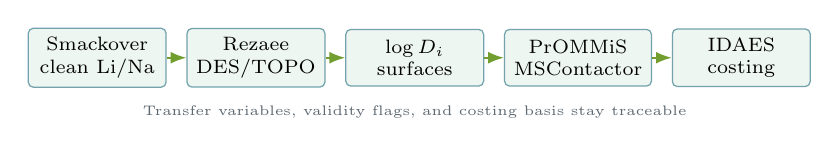
\begin{tikzpicture}[
      node distance=0.25cm,
      box/.style={
        rounded corners=1.8pt,
        draw=netlteal!60,
        fill=netlmist,
        line width=0.45pt,
        align=center,
        minimum width=1.75cm,
        minimum height=0.72cm,
        font=\scriptsize
      },
      arrow/.style={-{Latex[length=2mm]},line width=0.65pt,draw=netlgreen!80!netlnavy}
    ]
      \node[box] (feed) {Smackover\\clean Li/Na};
      \node[box,right=of feed] (reagent) {Rezaee\\DES/TOPO};
      \node[box,right=of reagent] (dist) {$\log D_i$\\surfaces};
      \node[box,right=of dist] (ms) {PrOMMiS\\MSContactor};
      \node[box,right=of ms] (cost) {IDAES\\costing};
      \draw[arrow] (feed) -- (reagent);
      \draw[arrow] (reagent) -- (dist);
      \draw[arrow] (dist) -- (ms);
      \draw[arrow] (ms) -- (cost);
      \node[font=\tiny,text=netlgray,align=center,below=0.12cm of dist] {Transfer variables, validity flags, and costing basis stay traceable};
    \end{tikzpicture}%
  }%
}

\newcommand{\costingplot}{%
  \begin{tikzpicture}
    \begin{axis}[
      width=0.94\linewidth,
      height=0.34\textheight,
      ybar=0pt,
      bar width=9pt,
      ymin=0,
      ymax=16,
      ylabel={\scriptsize USD/year, millions},
      symbolic x coords={Stress,Base,Favorable},
      xtick=data,
      tick label style={font=\scriptsize,text=netlnavy},
      label style={font=\scriptsize,text=netlgray},
      legend style={font=\tiny,draw=none,fill=none,at={(0.02,0.98)},anchor=north west},
      axis line style={netlgray!45},
      ymajorgrids,
      grid style={netlgray!12},
      nodes near coords,
      every node near coord/.append style={font=\tiny,rotate=90,anchor=west,text=netlnavy},
    ]
      \addplot[fill=netlteal!80,draw=netlteal] coordinates {(Stress,1.00) (Base,1.58) (Favorable,2.41)};
      \addplot[fill=netlgreen!85!netlnavy,draw=netlgreen!70!netlnavy] coordinates {(Stress,0.59) (Base,3.67) (Favorable,14.52)};
      \legend{annual cost,net before tax}
    \end{axis}
  \end{tikzpicture}%
}

\newcommand{\validationriskplot}{%
  \begin{tikzpicture}
    \begin{axis}[
      xbar,
      width=0.82\linewidth,
      height=0.43\textheight,
      xmin=0,
      xmax=450,
      xlabel={\scriptsize Na/Li mass ratio},
      symbolic y coords={Rezaee DOE max,MS-2 feed},
      ytick=data,
      tick label style={font=\scriptsize,text=netlnavy},
      label style={font=\scriptsize,text=netlgray},
      axis line style={netlgray!45},
      xmajorgrids,
      grid style={netlgray!12},
      nodes near coords,
      every node near coord/.append style={font=\scriptsize,text=netlnavy},
    ]
      \addplot[fill=netlteal!70,draw=netlteal] coordinates {(15,Rezaee DOE max)};
      \addplot[fill=netlwarning!90,draw=netlwarning] coordinates {(381.5,MS-2 feed)};
    \end{axis}
  \end{tikzpicture}%
}


\graphicspath{{figures/}}

\title{Produced-Water Lithium Extraction}
\subtitle{TBAC/DA DES + TOPO from Smackover feed basis to staged extraction and screening TEA}
\author{Chemical engineering technical review}
\institute{Smackover Li/Na feed basis $\rightarrow$ pretreatment $\rightarrow$ TBAC/DA DES + TOPO $\rightarrow$ ALAMO surrogate $\rightarrow$ PrOMMiS/IDAES}
\date{May 15, 2026}
\titlegraphic{\coverprocessmark}

\makeatletter
\@ifundefined{speakerNotes}{%
  \setbeameroption{hide notes}%
}{%
  \hypersetup{draft}%
  \setbeameroption{show notes on second screen=right}%
}
\makeatother

\newcommand{\DLi}{D_{\mathrm{Li}}}
\newcommand{\DNa}{D_{\mathrm{Na}}}
\newcommand{\SLiNa}{S_{\mathrm{Li/Na}}}
\newcommand{\sourcefoot}[1]{\vfill{\scriptsize\color{netlgray}#1}}
\newcommand{\slidetag}[1]{{\scriptsize\bfseries\color{netlteal}#1}\par\vspace{0.12cm}}
\newcommand{\sectiondivider}[1]{%
  \begin{frame}[plain,noframenumbering]
    \vspace*{0.42\textheight}
    {\Large\bfseries\MakeUppercase{#1}}\par
    \vspace{0.18cm}
    \begin{tikzpicture}
      \draw[netlgreen,line width=0.55pt] (0,0) -- (0.34\textwidth,0);
      \draw[netlgray!42,line width=0.45pt] (0.34\textwidth,0) -- (0.82\textwidth,0);
    \end{tikzpicture}
  \end{frame}
}

\newcommand{\transferpath}[1]{%
  \resizebox{#1\linewidth}{!}{%
    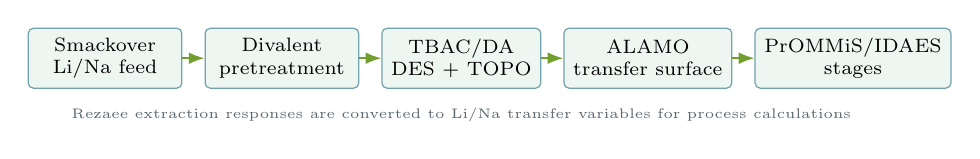
\begin{tikzpicture}[
      node distance=0.28cm,
      box/.style={
        rounded corners=1.8pt,
        draw=netlteal!60,
        fill=netlmist,
        line width=0.45pt,
        align=center,
        minimum width=1.95cm,
        minimum height=0.76cm,
        font=\scriptsize
      },
      arrow/.style={-{Latex[length=2mm]},line width=0.65pt,draw=netlgreen!80!netlnavy}
    ]
      \node[box] (feed) {Smackover\\Li/Na feed};
      \node[box,right=of feed] (pretreat) {Divalent\\pretreatment};
      \node[box,right=of pretreat] (solvent) {TBAC/DA\\DES + TOPO};
      \node[box,right=of solvent] (surrogate) {ALAMO\\transfer surface};
      \node[box,right=of surrogate] (process) {PrOMMiS/IDAES\\stages};
      \draw[arrow] (feed) -- (pretreat);
      \draw[arrow] (pretreat) -- (solvent);
      \draw[arrow] (solvent) -- (surrogate);
      \draw[arrow] (surrogate) -- (process);
      \node[font=\tiny,text=netlgray,align=center,below=0.12cm of solvent] {Rezaee extraction responses are converted to Li/Na transfer variables for process calculations};
    \end{tikzpicture}%
  }%
}

\newcommand{\stageplot}{%
  \begin{tikzpicture}
    \begin{axis}[
      width=0.92\linewidth,
      height=0.48\textheight,
      ymin=0,
      ymax=100,
      xlabel={\scriptsize solvent-extraction stages},
      ylabel={\scriptsize cumulative transfer, \%},
      xtick={1,3,5},
      tick label style={font=\scriptsize,text=netlnavy},
      label style={font=\scriptsize,text=netlgray},
      legend style={font=\tiny,draw=none,fill=none,at={(0.02,0.98)},anchor=north west},
      axis line style={netlgray!45},
      ymajorgrids,
      grid style={netlgray!12},
    ]
      \addplot[very thick,mark=*,color=netlteal] coordinates {(1,45.681) (3,83.770) (5,95.100)};
      \addplot[very thick,mark=square*,color=netlwarning] coordinates {(1,10.714) (3,29.008) (5,43.740)};
      \legend{Li recovery,Na co-transfer}
    \end{axis}
  \end{tikzpicture}%
}

\newcommand{\teaplot}{%
  \begin{tikzpicture}
    \begin{axis}[
      width=0.98\linewidth,
      height=0.44\textheight,
      ybar,
      bar width=11pt,
      ymin=0,
      ymax=19,
      ylabel={\scriptsize USD/kg LCE},
      xtick={1,2,3,4,5,6,7},
      xticklabels={Base,High Li,1 stage,5 stages,High pretreat,High solvent,Lower flow},
      x tick label style={font=\tiny,rotate=32,anchor=east,text=netlnavy},
      y tick label style={font=\scriptsize,text=netlnavy},
      label style={font=\scriptsize,text=netlgray},
      axis line style={netlgray!45},
      ymajorgrids,
      grid style={netlgray!12},
      nodes near coords,
      every node near coord/.append style={font=\tiny,text=netlnavy,rotate=90,anchor=west},
    ]
      \addplot[fill=netlteal!78,draw=netlteal] coordinates {
        (1,9.18)
        (2,6.11)
        (3,16.84)
        (4,8.09)
        (5,9.69)
        (6,9.75)
        (7,13.75)
      };
    \end{axis}
  \end{tikzpicture}%
}

\begin{document}

\begin{frame}[plain]
  \titlepage
  \note{
    Open by naming the purpose: this is an internal technical package for
    connecting Smackover produced-water chemistry to staged extraction and
    screening economics. Emphasize that the talk is about traceable integration:
    feed basis, pretreatment boundary, TBAC/DA DES + TOPO, ALAMO, PrOMMiS/IDAES,
    and TEA.
  }
\end{frame}

\begin{frame}[standout]
A pretreated Smackover Li/Na stream connects realistic produced-water chemistry
to staged extraction and screening-level economics.
\note{
  Use this as the one-sentence thesis. The audience should hear that the
  case study starts from a realistic produced-water feed, removes non-extraction
  burdens at the pretreatment boundary, and carries only Li/Na transfer variables
  into the process and cost layers.
}
\end{frame}

\section{Case Basis}
\sectiondivider{Case Basis}

\begin{frame}{Smackover Is The Main Produced-Water Case}
  \small
  \begin{columns}[T,onlytextwidth]
    \begin{column}{0.57\textwidth}
      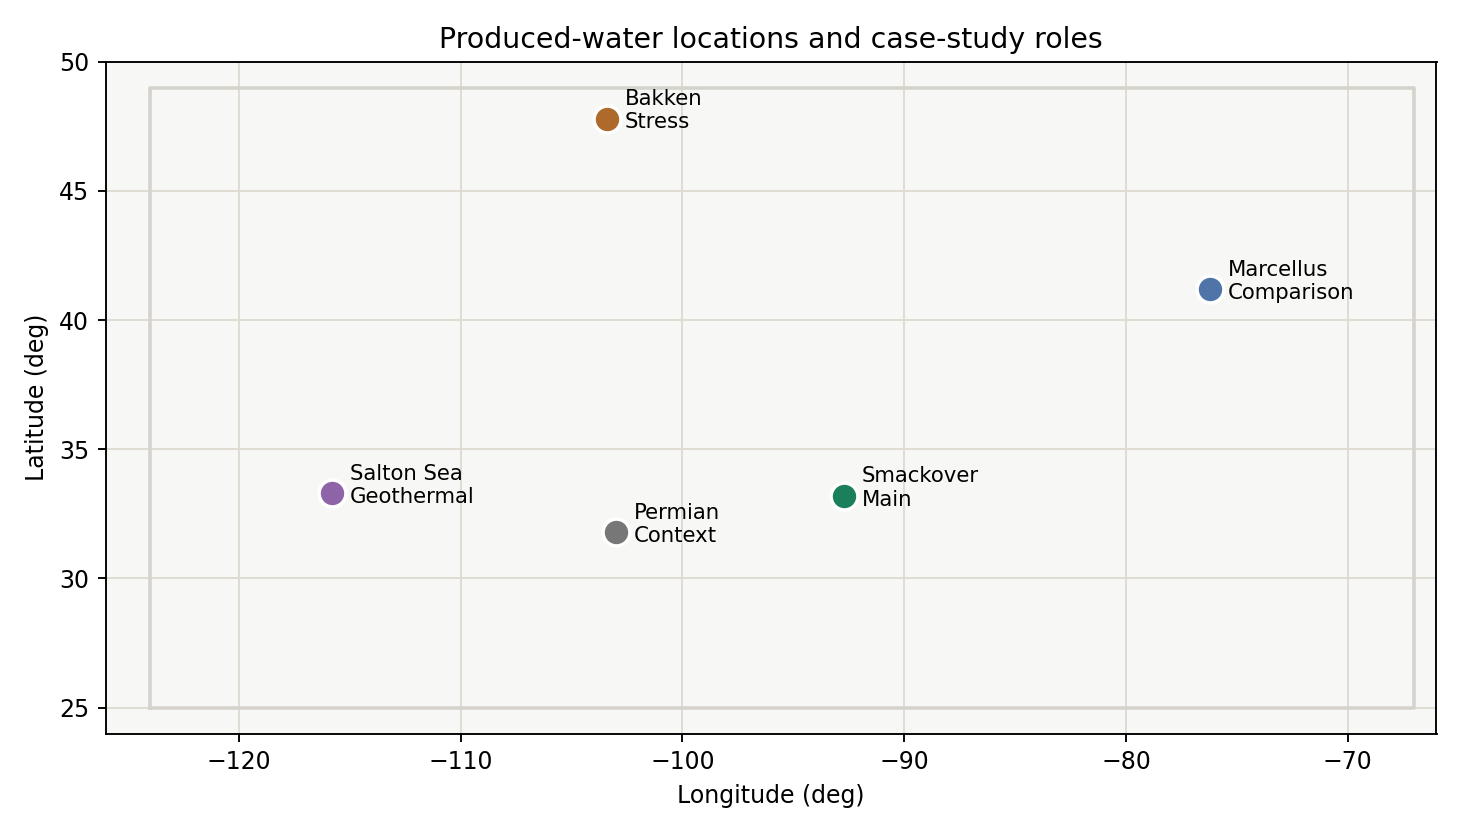
\includegraphics[width=\linewidth]{produced_water_basin_map.png}
    \end{column}
    \begin{column}{0.40\textwidth}
      \footnotesize
      \begin{alertblock}{Case basis}
        Southern Arkansas Smackover combines meaningful lithium grade with
        high-salinity major-ion chemistry.
      \end{alertblock}
      \begin{itemize}
        \item MS-2 feed: \SI{168}{mg/L} Li, \SI{64100}{mg/L} Na,
          and \SI{305000}{mg/L} TDS.
        \item High-observed Smackover sensitivity: \SI{252}{mg/L} Li.
        \item Marcellus, Bakken, Permian, and Salton Sea remain comparison cases.
      \end{itemize}
      \sourcefoot{Sources: USGS Smackover data release; selected feed table.}
    \end{column}
  \end{columns}
  \note{
    The point is not that Smackover is the only possible brine. It is the
    strongest primary case because it combines meaningful lithium with major-ion
    severity. The MS-2 row gives the main feed basis, and the high-Li Smackover
    row is kept as a clean sensitivity case rather than a new flowsheet.
  }
\end{frame}

\begin{frame}{Feed Variance Sets The Model Role}
  \begin{columns}[T,onlytextwidth]
    \begin{column}{0.61\textwidth}
      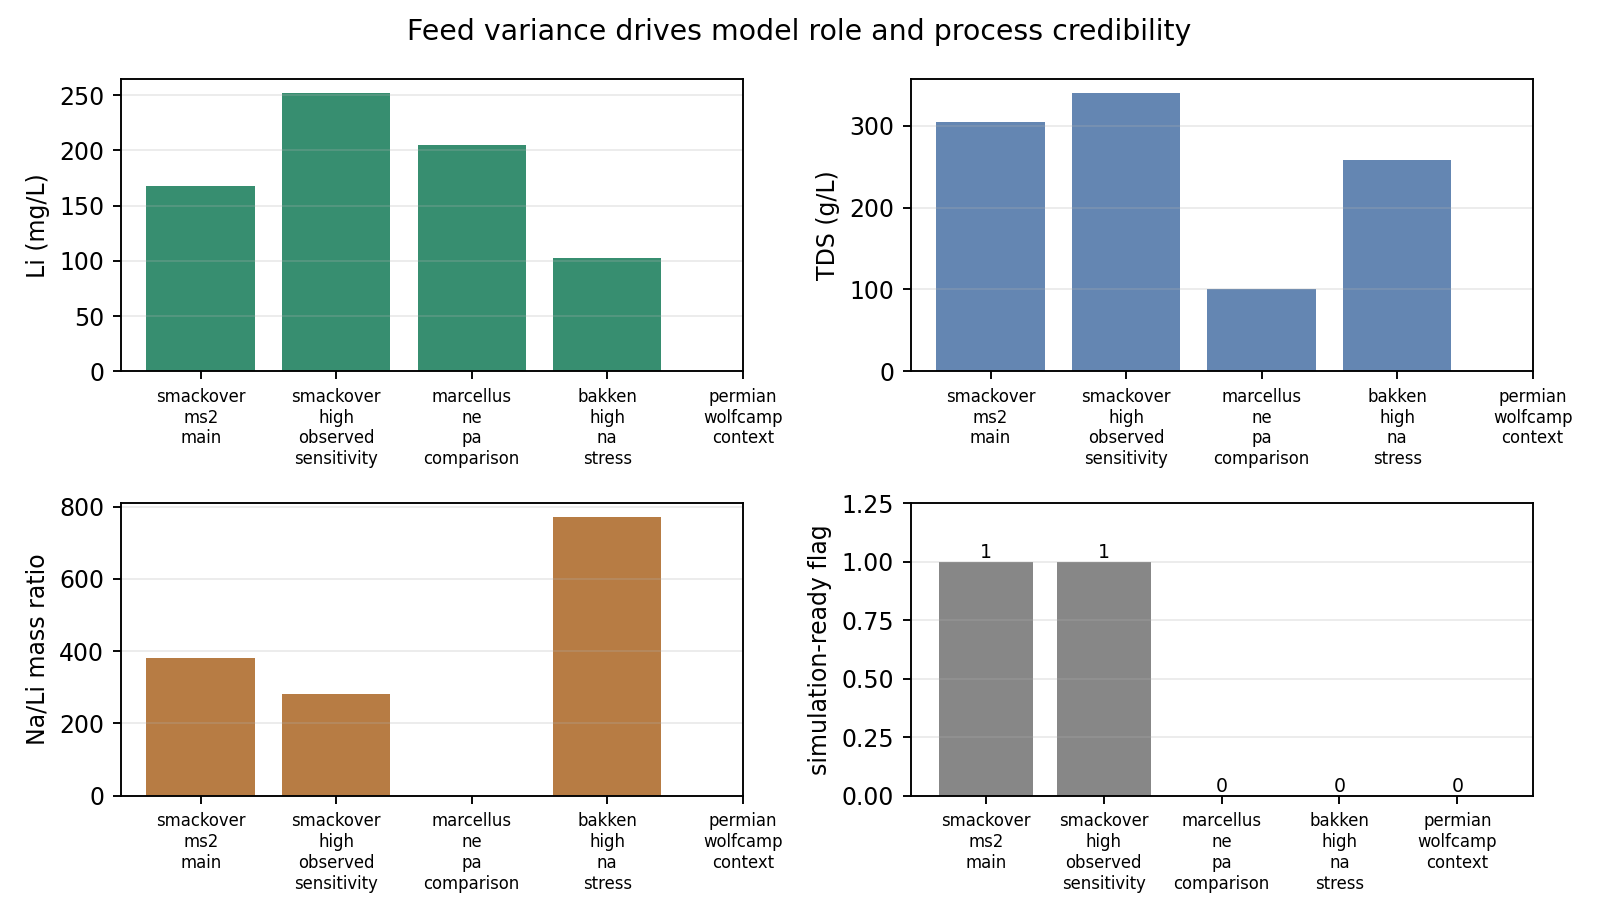
\includegraphics[width=\linewidth]{feed_variance_matrix.png}
    \end{column}
    \begin{column}{0.36\textwidth}
      \begin{itemize}
        \item Smackover MS-2 anchors the main flowsheet and TEA case.
        \item The high-Li Smackover row tests feed-grade sensitivity.
        \item Incomplete major-ion rows stay outside the main process calculation.
      \end{itemize}
      \vspace{0.2cm}
      \footnotesize
      \begin{tabular}{@{}ll@{}}
        \toprule
        Feed & Role \\
        \midrule
        MS-2 & main case \\
        High-Li Smackover & sensitivity \\
        Marcellus/Bakken & context \\
        \bottomrule
      \end{tabular}
    \end{column}
  \end{columns}
  \note{
    Explain why the model role is narrow. MS-2 is the case, high-Li Smackover is
    the feed-grade sensitivity, and the other basins provide context. This keeps
    the presentation from becoming a general produced-water survey while still
    showing why feed variance matters.
  }
\end{frame}

\begin{frame}{Pretreatment Creates The Li/Na Extraction Feed}
  \begin{columns}[T,onlytextwidth]
    \begin{column}{0.58\textwidth}
      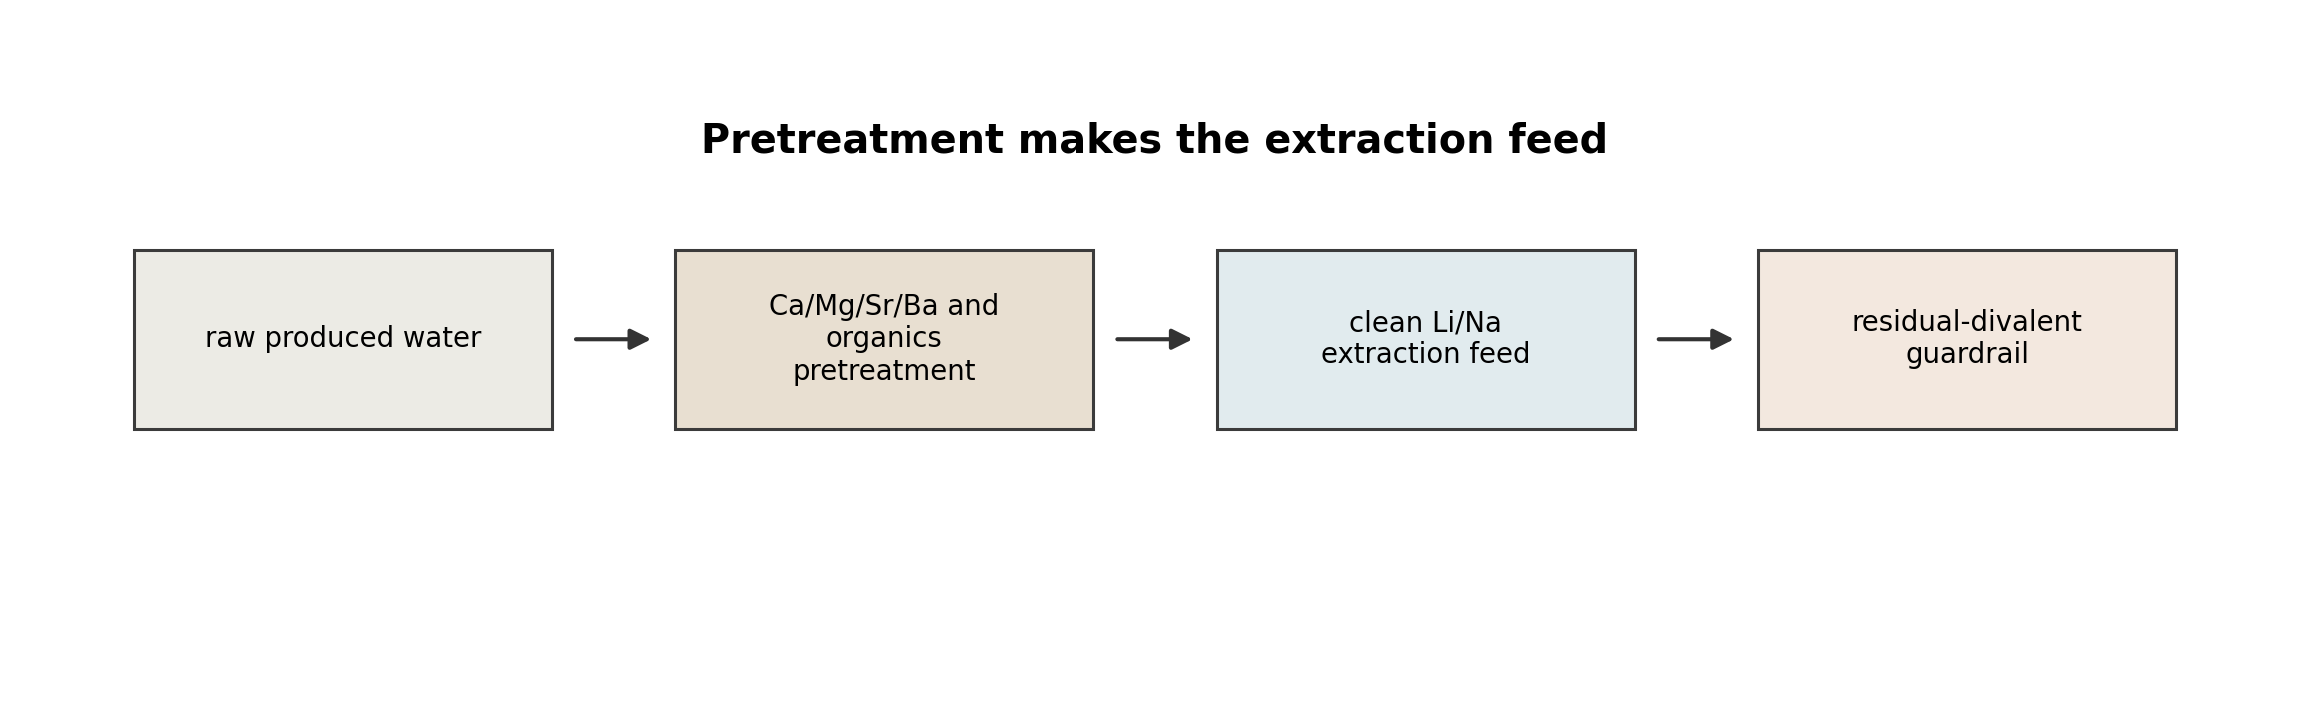
\includegraphics[width=\linewidth]{pretreatment_boundary.png}
    \end{column}
    \begin{column}{0.38\textwidth}
      \begin{itemize}
        \item Raw produced water is not the extraction feed.
        \item \ce{Ca^{2+}}, \ce{Mg^{2+}}, \ce{Sr^{2+}}, \ce{Ba^{2+}},
          suspended solids, oil, and organics are upstream treatment burdens.
        \item Lithium loss in pretreatment is carried into TEA sensitivity.
      \end{itemize}
    \end{column}
  \end{columns}
  \note{
    Say that raw produced water is not sent directly to the DES contactor. The
    extraction model receives a Li/Na feed after divalent removal and oil/solids
    handling. Pretreatment loss is still represented downstream in the TEA so the
    boundary is not free.
  }
\end{frame}

\section{Solvent And Transfer Surface}
\sectiondivider{Solvent And Transfer Surface}

\begin{frame}{TBAC/DA DES + TOPO Is The Active Solvent}
  \begin{columns}[T,onlytextwidth]
    \begin{column}{0.60\textwidth}
      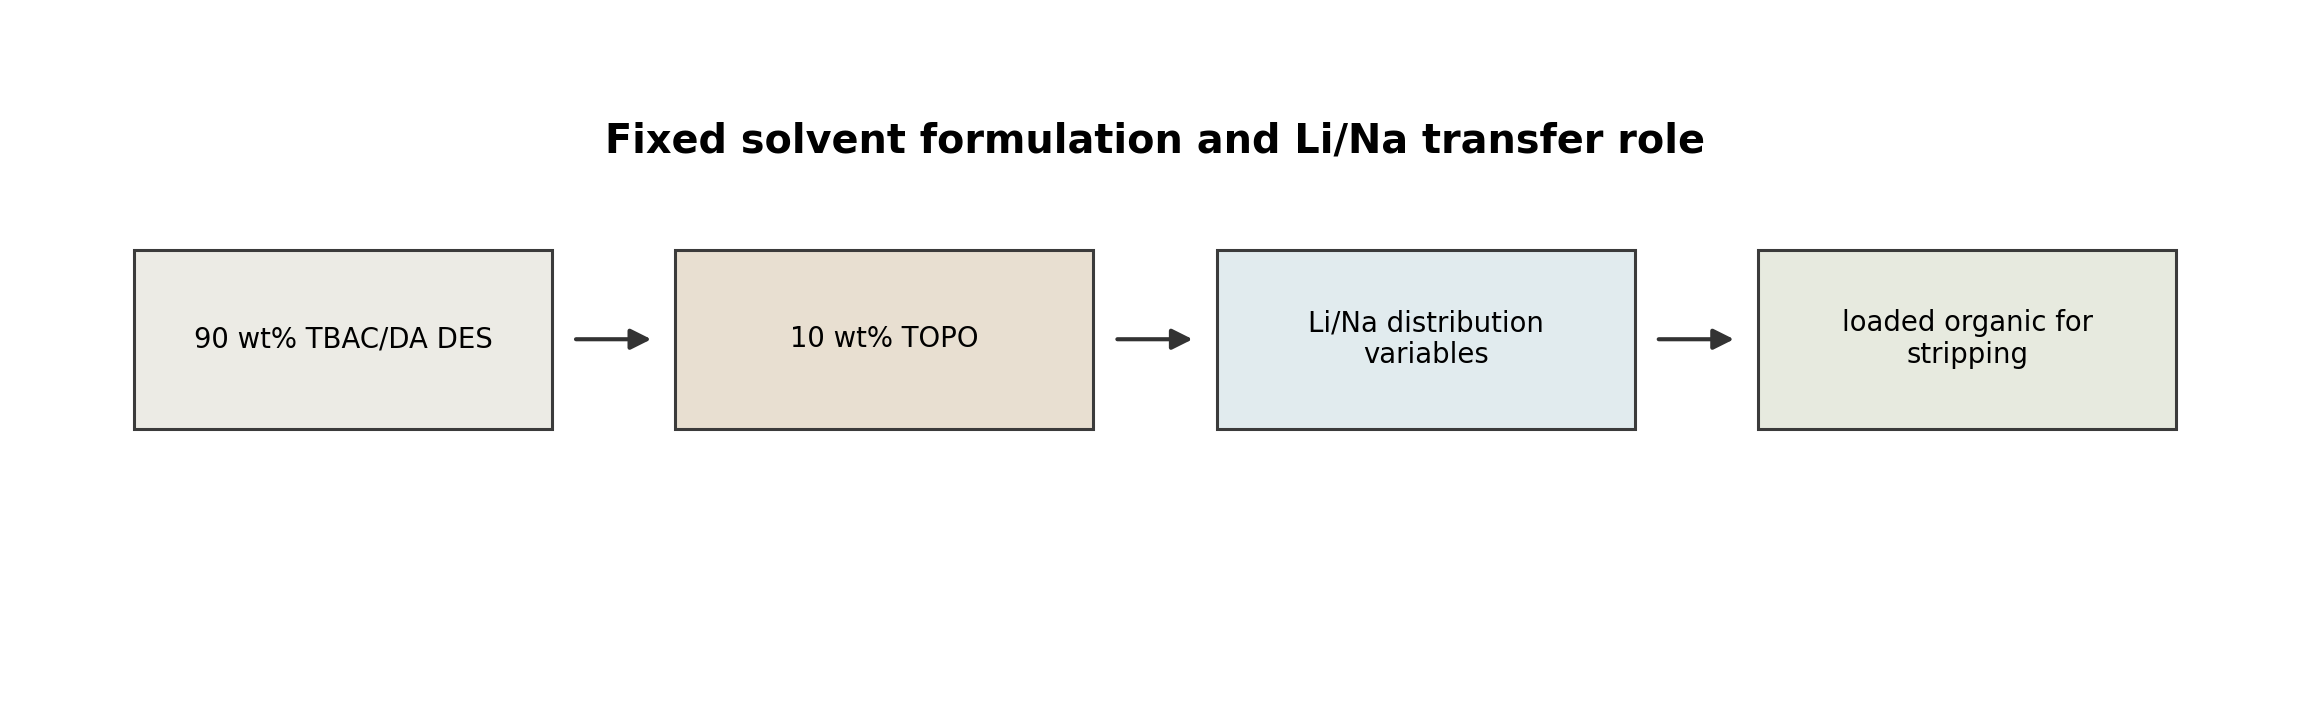
\includegraphics[width=\linewidth]{tbac_da_topo_mechanism.png}
    \end{column}
    \begin{column}{0.37\textwidth}
      \begin{itemize}
        \item Organic phase: 90 wt\% TBAC/DA DES and 10 wt\% TOPO.
        \item TBAC:DA molar ratio: 1:2.
        \item Temperature: \SI{23}{\celsius}.
        \item Aqueous pH: 10.4.
      \end{itemize}
      \sourcefoot{Source: Rezaee DES/TOPO extraction basis and supporting information.}
    \end{column}
  \end{columns}
  \note{
    This slide locks the chemistry. The active solvent is TBAC/DA DES with
    10 wt\% TOPO at the reported pH and temperature. Keep the message simple:
    the bridge is based on the Rezaee Li/Na extraction response for this solvent
    system, not a generic extractant screen.
  }
\end{frame}

\begin{frame}{Stage-Response Surface Spans Source And Smackover Domains}
  \small
  \begin{columns}[T,onlytextwidth]
    \begin{column}{0.54\textwidth}
      \footnotesize
      \begin{tabular}{@{}lrl@{}}
        \toprule
        Domain & Rows & Use \\
        \midrule
        source LHS & 625 & extraction anchors \\
        Smackover LHS & 625 & feed sensitivity \\
        reported anchors & 3 & Li/Na targets \\
        nominal/corner rows & 18 & stress bounds \\
        \bottomrule
      \end{tabular}
    \end{column}
    \begin{column}{0.42\textwidth}
      \begin{exampleblock}{Retained source anchors}
        \begin{tabular}{@{}lr@{}}
          optimized Li extraction & 48.57\% \\
          optimized Li/Na selectivity & 4.41 \\
          model-brine Li extraction & 51.63\% \\
          model-brine Na extraction & 9.97\% \\
        \end{tabular}
      \end{exampleblock}
      \begin{itemize}
        \item Reported extraction responses define the transfer anchors.
        \item Feed chemistry selects the Smackover case and validity bounds.
        \item The process calculation reports this paper-anchor transfer basis.
      \end{itemize}
    \end{column}
  \end{columns}
  \note{
    Walk through the table as the data contract. The source LHS and Smackover
    LHS span the response surface, and the reported anchors keep the model tied
    to the Rezaee extraction values. The important phrase is paper-response
    bridge: it is compact, traceable, and process-facing.
  }
\end{frame}

\begin{frame}{IDAES ALAMO Surrogate Preserves Li/Na Transfer Trends}
  \begin{columns}[T,onlytextwidth]
    \begin{column}{0.64\textwidth}
      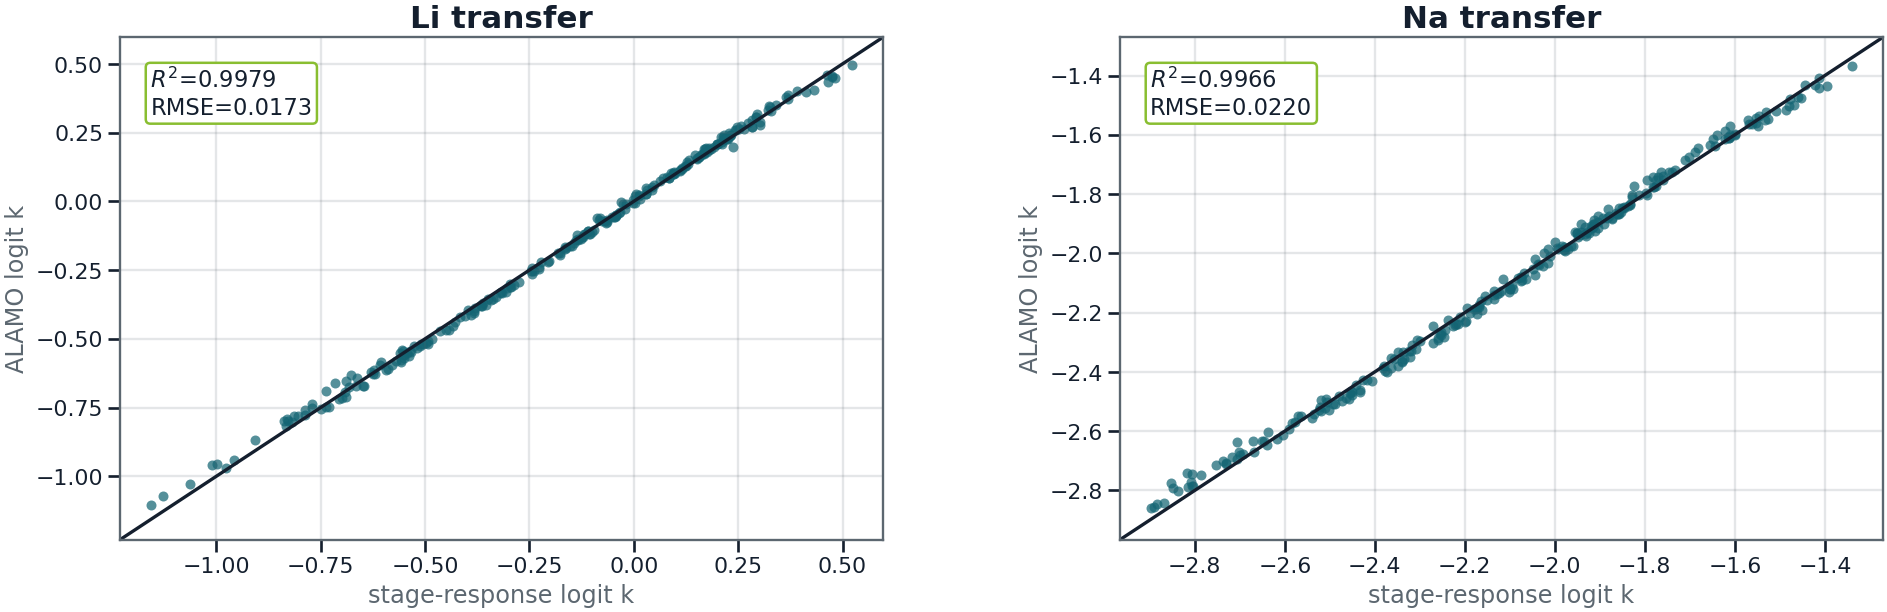
\includegraphics[width=\linewidth]{alamo_surrogate_parity_panel.png}
    \end{column}
    \begin{column}{0.32\textwidth}
      \footnotesize
      \begin{itemize}
        \item Inputs: Li concentration, Na concentration, O/A ratio, and TOPO loading.
        \item Outputs: logit-transformed Li and Na transfer coefficients.
        \item $R^2=0.9979$ for Li and $R^2=0.9966$ for Na on the held-out table.
      \end{itemize}
      \vspace{0.16cm}
      \begin{tabular}{@{}lcc@{}}
        \toprule
        Output & RMSE & max error \\
        \midrule
        logit $k_{\mathrm{Li}}$ & 0.0173 & 0.0555 \\
        logit $k_{\mathrm{Na}}$ & 0.0220 & 0.0779 \\
        \bottomrule
      \end{tabular}
    \end{column}
  \end{columns}
  \note{
    The ALAMO result is here to justify the compact transfer surface. The
    held-out parity is strong for both Li and Na in logit transfer space, so the
    surrogate is appropriate for the staged extraction calculations. Do not
    overstate this as a direct thermodynamic proof.
  }
\end{frame}

\begin{frame}{Paper-Response Variables Feed The Process Model}
  \begin{columns}[T,onlytextwidth]
    \begin{column}{0.48\textwidth}
      \[
        D_i = \frac{E_i}{100-E_i}\frac{1}{O/A}
      \]
      \[
        \SLiNa = \frac{\DLi}{\DNa}
      \]
      \begin{exampleblock}{Rezaee anchors, $O/A=1$}
        Optimized 10 wt\% TOPO:
        $E_{\mathrm{Li}}=48.57\%$, $\SLiNa=4.41$,
        so $E_{\mathrm{Na}}=11.01\%$.

        Model-brine row:
        $E_{\mathrm{Li}}=51.63\%$ and $E_{\mathrm{Na}}=9.97\%$.
      \end{exampleblock}
    \end{column}
    \begin{column}{0.49\textwidth}
      \transferpath{1.0}
    \end{column}
  \end{columns}
  \note{
    This is the equation slide for the process bridge. Extraction percent is
    converted to distribution coefficients, and Li/Na selectivity is the ratio
    of those coefficients. The Rezaee anchors give the numerical grounding; the
    flow diagram shows where the variables enter PrOMMiS/IDAES.
  }
\end{frame}

\section{Process And Economics}
\sectiondivider{Process And Economics}

\begin{frame}{PrOMMiS/IDAES Uses Active Li And Na Transfer Terms}
  \small
  \begin{columns}[T,onlytextwidth]
    \begin{column}{0.52\textwidth}
      \transferpath{1.0}
      \vspace{0.25cm}
      \begin{tabular}{@{}lrr@{}}
        \toprule
        Stages & Li recovery & Na co-transfer \\
        \midrule
        1 & 45.681\% & 10.714\% \\
        3 & 83.770\% & 29.008\% \\
        5 & 95.100\% & 43.740\% \\
        \bottomrule
      \end{tabular}
    \end{column}
    \begin{column}{0.44\textwidth}
      \begin{itemize}
        \item The process layer uses PrOMMiS \texttt{SolventExtraction} objects
          with IDAES \texttt{MSContactor} units.
        \item Lithium and sodium material-transfer terms are active.
        \item Chloride transfer is held at zero inside the Li/Na extraction boundary.
      \end{itemize}
    \end{column}
  \end{columns}
  \note{
    Emphasize the process-model handoff: Li and Na transfer are active terms,
    while chloride is held outside the extraction boundary. The staged results
    are not a standalone chemistry claim; they are what happens when the
    paper-response transfer variables are carried into the PrOMMiS/IDAES stage
    structure.
  }
\end{frame}

\begin{frame}{Three Stages Recover 83.77\% Lithium}
  \begin{columns}[T,onlytextwidth]
    \begin{column}{0.61\textwidth}
      \stageplot
    \end{column}
    \begin{column}{0.36\textwidth}
      \begin{itemize}
        \item Smackover MS-2 at $O/A=1$ and 10 wt\% TOPO reaches
          83.77\% cumulative lithium recovery after three stages.
        \item Sodium co-transfer is 29.01\% at the same condition.
        \item Five stages raise lithium recovery to 95.10\% with a larger
          sodium burden.
      \end{itemize}
    \end{column}
  \end{columns}
  \note{
    This is the recovery slide. One stage gives the first extraction step, three
    stages is the main design point, and five stages shows the recovery ceiling
    with higher sodium co-transfer. The 83.77\% number is the main process result
    to carry forward into the TEA.
  }
\end{frame}

\begin{frame}{Screening TEA Centers At 9.18 USD/kg LCE}
  \begin{columns}[T,onlytextwidth]
    \begin{column}{0.62\textwidth}
      \teaplot
    \end{column}
    \begin{column}{0.35\textwidth}
      \begin{itemize}
        \item Base Smackover intensity is 9.18 USD/kg lithium carbonate equivalent.
        \item High-Li feed sensitivity lowers the value to 6.11 USD/kg.
        \item One stage raises the value to 16.84 USD/kg through lower recovery.
      \end{itemize}
    \end{column}
  \end{columns}
  \note{
    Present the TEA as screening-level prioritization. The base case is
    9.18 USD/kg LCE, high feed grade moves the number down, and one stage moves
    it up by losing recovery. The value of the slide is ranking the levers, not
    claiming plant cost certainty.
  }
\end{frame}

\begin{frame}{Economic Levers Are Feed Grade, Stages, And Losses}
  \scriptsize
  \begin{columns}[T,onlytextwidth]
    \begin{column}{0.58\textwidth}
      \resizebox{\linewidth}{!}{%
      \begin{tabular}{@{}lrrr@{}}
        \toprule
        Scenario & Recovery & Cost & p10--p90 \\
        \midrule
        base Smackover & 79.58\% & 9.18 & 8.81--12.43 \\
        high-Li Smackover & 79.72\% & 6.11 & 5.92--8.26 \\
        one stage & 43.40\% & 16.84 & 16.15--22.52 \\
        five stages & 90.35\% & 8.09 & 7.77--10.74 \\
        high pretreatment loss & 75.39\% & 9.69 & 8.93--12.57 \\
        high solvent loss & 79.58\% & 9.75 & 9.00--12.59 \\
        lower throughput & 79.58\% & 13.75 & 12.65--18.96 \\
        \bottomrule
      \end{tabular}
      }%
      \sourcefoot{Cost values in USD/kg lithium carbonate equivalent.}
    \end{column}
    \begin{column}{0.38\textwidth}
      \begin{alertblock}{Screening boundary}
        The TEA compares operating sensitivities for prioritization; it does not
        replace equipment design, residence-time sizing, solvent-loss experiments,
        or product-pricing analysis.
      \end{alertblock}
      \begin{itemize}
        \item Feed lithium grade is the strongest favorable lever.
        \item Stage count trades lithium recovery against sodium loading.
        \item Fixed annual charges dominate the lower-throughput case.
      \end{itemize}
    \end{column}
  \end{columns}
  \note{
    Use this slide to explain tradeoffs. Better lithium grade and enough stages
    improve cost intensity; pretreatment loss, solvent loss, and lower throughput
    move the result in the wrong direction. The p10--p90 band is useful for
    showing that feed and stage choices dominate the screening sensitivity.
  }
\end{frame}

\section{Thermodynamic Extension}
\sectiondivider{Thermodynamic Extension}

\begin{frame}{Case-Study Coverage Matrix}
  \scriptsize
  {\setlength{\tabcolsep}{3pt}\renewcommand{\arraystretch}{1.23}
  \begin{tabular}{@{}>{\raggedright\arraybackslash}p{0.20\textwidth}>{\raggedright\arraybackslash}p{0.34\textwidth}>{\raggedright\arraybackslash}p{0.36\textwidth}@{}}
    \toprule
    Lane & Current basis & Process-facing use \\
    \midrule
    feed basis & Smackover MS-2 and high-Li Smackover sensitivity &
      defines the main and feed-grade sensitivity cases \\
    paper-response bridge & Rezaee Li/Na extraction responses with $O/A$
      conversion & supplies $\DLi$, $\DNa$, and $\SLiNa$ for staged extraction \\
    ALAMO surrogate & held-out parity for logit $k_{\mathrm{Li}}$ and logit
      $k_{\mathrm{Na}}$ & provides the compact transfer surface used by the
      process model \\
    PrOMMiS/IDAES stages & PrOMMiS/IDAES staged-extraction terms for Li and Na
      across 1, 3, and 5 stages & converts transfer variables to outlet
      recovery and raffinate behavior \\
    screening TEA/UQ & feed grade, stage count, pretreatment loss, solvent
      loss, and throughput & ranks operating levers for sprint approval \\
    direct ePC-SAFT replacement path & accepted Li/Na transfer rows & replaces
      the paper-response bridge without changing process inputs \\
    \bottomrule
  \end{tabular}}
  \vspace{0.14cm}
  {\footnotesize\color{netlgray}
  Process-facing rows remain stable as the thermodynamic basis is exchanged.}
  \note{
    This is the scope-control slide. The current package covers the feed basis,
    paper-response bridge, ALAMO surrogate, PrOMMiS/IDAES stages, and screening
    TEA/UQ. For interim ePC-SAFT support, cite the Rezaee 2026 26-row
    reactive-equilibrium replay: the package evaluates the aqueous ePC-SAFT and
    organic PC-SAFT activity terms, and the calibrated actual-row replay has
    median $\ln Q-\ln K$ offsets of -0.23 for Li and 0.20 for Na. That supports
    the replacement path, but it is not a direct Li/Na transfer-row result.
  }
\end{frame}

\begin{frame}[standout]
The case study is a screening-quality bridge from Smackover feed chemistry to
PrOMMiS/IDAES staged extraction and TEA, ready to anchor an internal
ePC-SAFT-to-PrOMMiS/IDAES integration sprint.
\note{
  Say the ask plainly: approve a focused internal sprint that connects accepted
  ePC-SAFT Li/Na transfer rows to the existing PrOMMiS/IDAES interface. The deck
  is already organized so the paper-response bridge can be exchanged without
  changing the process inputs.
}
\end{frame}

\begin{frame}{Technical Message}
  \begin{enumerate}
    \item Smackover MS-2 is the main produced-water feed; the high-Li Smackover
      row defines the feed-grade sensitivity.
    \item TBAC/DA DES + 10 wt\% TOPO maps lithium and sodium transfer through
      ALAMO and into staged solvent extraction.
    \item Three stages recover 83.77\% lithium before the TEA pretreatment-loss
      adjustment.
    \item The base screening TEA is 9.18 USD/kg LCE, with feed grade and stage
      count controlling the largest movement.
    \item Ask: approve an internal ePC-SAFT-to-PrOMMiS/IDAES integration and
      validation sprint.
  \end{enumerate}
  \note{
    Read this slide as the closing script. The first four bullets summarize the
    technical chain and the fifth bullet is the decision request. If asked about
    current ePC-SAFT data, use the results folder carefully: it supports
    Rezaee-style activity-term replay and calibrated actual rows, while direct
    transfer rows remain the next accepted input to the process bridge.
  }
\end{frame}

\begin{frame}{Supplemental Extension Context}
  \scriptsize
  {\setlength{\tabcolsep}{3pt}\renewcommand{\arraystretch}{1.24}
  \begin{tabular}{@{}>{\raggedright\arraybackslash}p{0.18\textwidth}>{\raggedright\arraybackslash}p{0.36\textwidth}>{\raggedright\arraybackslash}p{0.36\textwidth}@{}}
    \toprule
    Family & Why it belongs near produced water & Needed before modeling \\
    \midrule
    CMM/REE ions & oilfield brines can carry critical-mineral value beyond Li
      & measured composition, aqueous speciation, and ion parameters \\
    divalent ions & Ca, Mg, and Sr set pretreatment load and leakage risk &
      pretreatment data and extraction leakage bounds \\
    hydrocarbons & oil-bearing water adds phase behavior and solvent-contact
      risks & oil-phase assay and phase-equilibrium data \\
    ePC-SAFT extension & electrolyte and Born/dielectric terms give a
      thermodynamic route & accepted parameters and phase data for each species
      family \\
    \bottomrule
  \end{tabular}}
  \vspace{0.26cm}
  \begin{columns}[T,onlytextwidth]
    \begin{column}{0.48\textwidth}
      \begin{block}{Boundary}
        Li/Na extraction remains the present case. CMM, REE, and hydrocarbon
        rows define where additional data would expand the same structure.
      \end{block}
    \end{column}
    \begin{column}{0.48\textwidth}
      \begin{exampleblock}{Use}
        The extension list guides what to measure before adding species,
        reactions, or oil-phase terms to the thermodynamic model.
      \end{exampleblock}
    \end{column}
  \end{columns}
  \sourcefoot{USGS Energy Waste Science; critical-mineral produced-water review; electrolyte PC-SAFT permittivity and ePC-SAFT Born/dielectric literature.}
  \note{
    Keep this slide supplemental. It says CMM, REE, divalent ions, and
    hydrocarbons are natural produced-water extensions, but each needs measured
    composition, phase data, parameters, and extraction chemistry before joining
    the case study. Do not imply these systems are already solved by the Li/Na
    model.
  }
\end{frame}

\begin{frame}{Sources}
  \begin{itemize}
    \item Rezaee et al. 2025: TBAC/DA DES + TOPO extraction response basis.
    \item Rezaee et al. 2026: PC-SAFT/ePC-SAFT parameter and reaction-equilibrium support.
    \item U.S. Geological Survey southern Arkansas Smackover brine data release,
      DOI: \texttt{10.5066/P9QPRYZN}.
    \item USGS Energy Waste Science and produced-water lithium/mineral recovery context.
    \item Critical-mineral source potential review for U.S. oil and gas
      produced waters.
    \item Electrolyte PC-SAFT permittivity and ePC-SAFT Born/dielectric
      literature for the extension basis.
    \item Produced-water feed table, ALAMO validation table, PrOMMiS/IDAES
      staged-extraction table, and screening TEA table from the case-study result tables.
  \end{itemize}
  \note{
    Use sources only if the audience asks where the basis comes from. Rezaee
    supplies extraction and thermodynamic-modeling inputs, USGS supplies the
    produced-water context, and the case-study result tables supply the bridge,
    stage, and TEA values used in the deck.
  }
\end{frame}

\end{document}
